%\documentclass[a4paper,10pt]{article}
\documentclass[10pt, conference, letterpaper]{IEEEtran}
\usepackage[utf8]{inputenc}
\usepackage{xspace}
\usepackage{url}
\usepackage{graphicx,graphics} 
\usepackage{color}
\usepackage{amsmath}
\usepackage{amsfonts}
\usepackage{amssymb}
\usepackage{amsthm}
\usepackage{algorithm}
\usepackage{algorithmic}
\usepackage{longtable}
\usepackage{complexity}
\usepackage{tkz-graph}
\usepackage{float}
\usepackage{tabularx}
\usepackage{setspace}
\usepackage{icomma}
\usepackage{complexity}
\renewcommand{\algorithmicrequire}{\textbf{Input:}}
\renewcommand{\algorithmicensure}{\textbf{Output:}}
\usepackage{authblk}
\usepackage[colorlinks=true,breaklinks=true,linkcolor=blue]{hyperref}


\newtheorem{proposition}{Proposition}
\newtheorem{theorem}{Theorem}

\setlength{\parskip}{1ex} % Espace entre les paragraphes

\newtheorem{fact}{Fact}
\newtheorem{lemma}[theorem]{Lemma}
\newtheorem{definition}{Definition}
\newtheorem{corollary}{Corollary}

% \renewcommand{\thefootnote}{\*}

\newcommand\pma{\textsc{pma}\xspace}

\title{Scheduling periodic messages and their answers on a single link}
 

\author[1,2]{Ma\"el Guiraud}
\author[1]{Yann Strozecki}
\affil[1]{David Laboratory, UVSQ}
\affil[2]{Nokia Bell Labs France}

\begin{document}

\maketitle

\begin{abstract}

A recent trend in mobile networks is to centralize in distant data-centers processing units which, until now, were attached to antennas. The main challenge is to guarantee a low latency for the periodic messages sent from the antennas to their processing units and back  to fulfill protocol time constraints. The problem we adress is to find a sending scheme from the antennas to their processing units and back without contention nor buffering.

We focus on a simple but common star shaped topology, where all contentions are on a single arc shared by all antennas. For messages of arbitrary size, we show that there is always a solution as soon as the load of the network is less than $40\%$. Moreover, we explain how we can restrict our study to packet of size $1$ without increasing too much the global latency. 

For message of size $1$, we prove that it is always possible to schedule them on a star shaped topology, when the load is less than $2/3$ using a polynomial time algorithm.
Moreover, using a simple random greedy algorithm, we show that almost all
instances of a given load admit a solution, explaining why most greedy algorithms work so well in practice.  
\end{abstract}


\section{Introduction}

Lister les usages possibles: 
sans retour mais de profondeur 2 ou plus. Sonar ? Train ?
Réseau de capteurs communicant (industrie)
Logistique dans une usine (chaine avec différent produits)

Comparer à la litérature. Aller voir ce qu'on nous a cité sur l'ordonnancement périodique 
et les trucs de train périodique qu'on a trouvé.
Dire que c'est du scheduling : contention point = machine et message = task.


Mélanger l'introduction et le modèle. Voir comment c'est présenté dans two flow shop

In this article, we model a very simple network in which periodic messages flow through a single link. The answer to each message is then sent back through the same bidirectional link. The model and problem can easily be generalized to any network, that is any directed acyclic graph with any number of contention points, see \cite{dominique2018deterministic}. We choose here to present the simplest non trivial such network, for which we can still obtain some theoritical results. 

The time is discretized and the process we consider is periodic of fixed integer period $P$. We use the notation $[P]$ for the set $\{0,\dots,P-1\}$. In our application, all messages are of the same nature, hence they are all of the same size denoted by $\tau$. This size corresponds to the time it requires to send it through some contention point of the network.
We denote by $n$ the number of messages, which are numeroted from $0$ to $n-1$. A message $i$ is caracterized by its delay $d_i$. It means that if the message number $i$ goes in the link at time $t$, then it returns to it in the other direction at a time $t + d_i$. 
\begin{center}
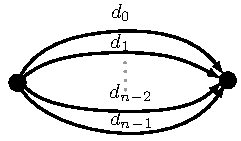
\includegraphics{distances}
\end{center}
Since the process we describe is periodic, we chose any interval of $P$ unit of time.
Describing the messages going through the two contention points during such an interval
completely define the periodic process. We call the representation of the interval
of time in the first contention point the \emph{first period} and the \emph{second period}
for the second contention point.

An \emph{offset} of a message is a choice of time at which it arrives
at the first contention point. Let us consider a message $i$
of offset $o_i$, it uses the interval of time $[i]_1 = \{ (o_i + t) \mod P \mid 0 \leq t < \tau \}$ in the first period and $[i]_2 = \{ (d_i + o_i + t) \mod P \mid 0 \leq t < \tau \}$ in the second period. We say that two messages $i$ and $j$ collide if either $[i]_1 \cap [j]_1 \neq \emptyset $ or $[i]_2 \cap [j]_2 \neq \emptyset $.

We want to send all messages, so that they are no collision in the common link.
In other word, we look for a way to send the messages without using buffering and 
hence limiting the latency to the physical length of the link. An assignment is a
choice of an offset for each message such that \emph{no pair of message collide}.
Formally, an \emph{assignment} is a function from the messages, represented by their indices in $[n]$ to their offsets in $[P]$.  

We call Periodic Message Assignment or \pma the problem we study in this article,
which asks, given an instance of $n$ messages, a period $P$ and a size $\tau$ to find 
an assignment or to decide there is none.
\begin{center}
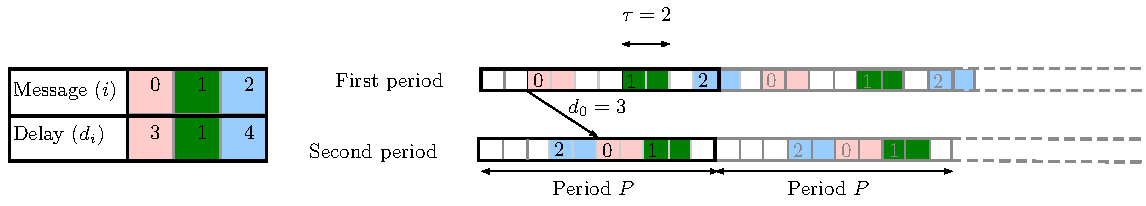
\includegraphics[scale=0.7]{instance}
\end{center}
The complexity of \pma is not known. However, we have proven that when parametrized by
$n$ the number of messages, the problem is \FPT~\cite{barth2018deterministic}.
A slight generalization of \pma, with several contention points but each message only goes through two as in \pma is \NP-hard~\cite{barth2018deterministic}. If the the link is not bidirectional, that is there is a single contention point and each message goes through it twice, it is also \NP-hard~\cite{}. Hence, we conjecture that \pma is \NP-hard.

To overcome the hardness, we study \pma in this article when the load of the system is small enough. The \emph{load} is defined as the number of unit of time used in a period by messages in a contention point divided by the period. Hence the load is equal to $n\tau /P$.
Our aim is to prove that for small load, there is \emph{always} an assignment and that it can be found by a polynomial time algorithm.


\section{Greedy Algorithms for Large Messages}

In this section, we study the case of large messages. When modelizing real problems,
it is relevant to have $\tau > 1$ when the transmission time of a single message is large with regard to its delay.


A partial assignment $A$ is a function defined from a subset $S$ of $[n]$ to $[P]$.
We say that $|S|$, the cardinal of the domain of $A$, is its \emph{size}.
We say that a message in $S$ is \emph{scheduled} (by $A$), and a message not in $S$ is \emph{unscheduled}. We only consider partial assignments such that no pair of messages of $S$ collide. If $A$ has domain $S$, and $i \notin S$, we define the extension of $A$ to the message $i$ by the offset $o$, denoted by $A[i \rightarrow o]$, the function defined as $A$ on $S$ and $A[i \rightarrow o](i) = o$.

All presented algorithms build the assignment incrementally, by growing the size of the domain of a partial assignment. Moreover, the algorithm of this section are greedy since once an offset is chosen for a message, it is never changed.


\subsection{First fit}


Assume that for some partial assignment $A$, the message $i$ has offset $o$: it uses all times from $o$ to $o + \tau -1$ in the first period. If a message $j$ is scheduled with some offset $o'$ before $o$, then the last time it uses in the first period is $o'+\tau-1$ and it should be less than $o$, which implies that $o' \leq o - \tau + 1$. If $o'$ is larger than $o$, to avoid collision between messages $j$ and $i$, it should be larger or equal to $o+ \tau$. Hence the message $i$ forbids $2\tau -1$ positions for messages still not scheduled because of tis use of time in the first period. The same reasonning can be done for the second period, wich again forbids $2\tau -1$ offsets. Hence, if $|S|$ messages are already scheduled, then $|S|(4\tau -2)$ offsets are forbidden for the an unscheduled messages. Note that this is an upper bound on the number of forbidden offsets, since the same offset can be forbidden because of a message on the first and also on the second period.

We define $Fo(A)$, the maximum number of forbidden offsets when 
extending $A$. Formally, assume $A$ is defined over $S$ and $i\notin S$, 
it is the maximum over all values of $d_i$ of $|\left\{ o \in [P] \mid A[i \rightarrow o] \text{ has no collision }\right\}|$. The previous paragraph shows that $Fo(A)$ is always bounded by $(4 \tau -2)|S|$. 

The first algorithm deals with the route in the order they are given:  for each unscheduled route it tests all offsets from $0$ to $P-1$ until one do not create a collision with the current assignment.
We call this algorithm \emph{First Fit}. Remark that if $Fo(A) < P$, then whatever the delay of the route we want to extend $A$ with, it is possible to find an offset. Since $Fo(A) \leq (4 \tau -2)|S|$ and $|S| < n$, First Fit (or any greedy algorithm) will always succed 
when $(4 \tau -2)n \leq P$, that is when $ n\tau /P \leq 1/4$.
It turns out that First Fit always create compact assignments (as defined in~\cite{barth2018deterministic}), that is a message is always next to another one in one of the two period. Hence, we can prove a better bound on $Fo(A)$, when $A$ is built by First Fit, which
implies the following therem.

\begin{theorem}
First Fit always solves \pma positively on instances of load less than $1/3$. 
\end{theorem}
\begin{proof}
To prove the theorem, e prove that by induction on the size of $S$ that $Fo(A) \leq |S|(3\tau -1) + \tau -1$.  For $S = 1$, it is clear since a single message forbid at most $(3\tau -1) + \tau -1 = 4\tau-2$ offsets, as explained before. Now, assume $Fo(A) \leq |S|(3\tau -1) + \tau -1$ and consider a route $i \notin S$ such that First Fit builds $A[i \rightarrow o]$ from $A$. By definition of First Fit, choosing $o-1$ as offset creates a collision, w.l.o.g. 
say it is a collision in the first period. It means that there is a shceduled message between $o - \tau $ and $o-1$ (modulo $P$), hence all these offsets are forbidden by $A$.
The same offsets are also forbidden by the choice of $o$ as offset for $i$, then only $3\tau -1$ new offsets are forbidden, that is $Fo(A[i \rightarrow o]) \leq Fo(A) + (3\tau -1)$,
which proves the induction and the theorem.
\end{proof}

\subsection{Meta-intervals}

The second method is described  in~\cite{barth2018deterministic} and achieves the same bound on the load using a different method which is also be used in the more involved algorithms
of the next section.
The idea is to restrict the possible offsets at which messages can be scheduled. It seems counter-intuitive, since it decreases artificially the number of possible offsets to schedule new messages. However, it allows to reduce the number of forbidden offsets, when the algorithm is designed accordingly. A \emph{meta-offset} is an offset of value $i\tau$,
with $i$ an integer from $0$ to $P / \tau$. We call Meta-Offset the greedy algorithm
which works as First Fit, but consider only meta-offsets when scheduling new messages. 

We define $Fmo(A)$ as the maximal number of meta-offsets forbidden by $A$. 
 By definition, two messages with a different meta-offset cannot collide in the first period.
Hence, $Fmo(A)$ can be bounded by $3|S|$ and we obtain the following theorem.


\begin{theorem}[Proposition 3 of~\cite{barth2018deterministic} ]
Meta-Offset always solves \pma positively on instances of load less than
$1/3$.
\end{theorem}

\subsection{Tuples and meta-intervals}

We now propose a more involved family of greedy algorithms which 
solves \pma positively for larger loads. We try to combine the good properties of the two previous algorithms: the compacity of the solutions of the first one and the use of meta-offsets ofthe second algorithm to reduce collisions on the first period.
The idea is to schedule several messages at once, using meta-offsets, to maximize the compacity of the obtained solution. 


We first describe the algorithm which places pairs of routes and then explain quickly how we can extend it by placing tuples of messages instead of pairs.

We first needs a lemma which allows to assume that the period $P$ is a multiple of $\tau$, 
which makes the analysis of our algorithms much simpler and tighter. It only changes the load
from $n \tau / P$ to at most $n (\tau +1)/ P$: the difference is less than $n /P < 1/\tau$,
and is very small for large $\tau$.

\begin{lemma}
Let $I$ be an instance of \pma with $n$ messages of size $\tau$ and period $P$.
Let $m = P / \tau$. There is an instance $I'$ with $n$ messages of size $\tau'$ and period $P'= m\tau'$ such that an assignment of $I'$ can be transformed into an assignment of $I$.
\end{lemma}
\begin{proof}
Let $P = m \tau + r$ with $r \leq \tau$. We define the instance $I'$ as follows: $P' = mP$, $d_{i}' = m d_i$ and $\tau' = m \tau + r$. With this choice, we have $P' = m(m \tau + r) = m \tau'$.
Consider an assignment $A'$ of the instance $I'$.
If we let $\tau'' = m\tau$, then $A'$ is also an assignment for $I'' = (P',\tau'',(d_{0}',\dots,d_{n-1}'))$ since we only reduce the size of each message (the interval of time used in the first and second period begi at the same position but are shorter).
We then use a compactification procedure as in~\cite{barth2018deterministic}. The first message is positionned at offset zero. The first time it uses in the second period is a multiple of $m$ since its delay is by definition a multiple of $m$. Then all the other messages are translated to the left until there is a collision (remove increasing values from all offsets but the offset of the first message). It guarantees that some message is in contact with the first one,  which implies that its offset is a multiple of $m$. This procedure can be repeated until we get some solution $A''$ to $I''$, and by induction it is proven that all positions of messages in the first and second period are multiple of $m$. Hence, if we define $A$ as $A(i) = A''(i)/m$, we obtain an assignment of $I$.
\end{proof}

From now on, we always assume that $P = m\tau$ and the load is then $n/m$.
We are interested in the remainder modulo $\tau$ of the delays of each message.
We write $d_i = d_{i}'\tau + r_i$ and assume from now on that messages are sorted by increasing $r_i$.
A \emph{compact pair} is a pair of messages $(i,j)$ with $i < j$ such that we can put them
next to each other in the second period using meta-offsets.
We have $r_i \leq r_j$ since $i < j$. We denote by $g$ the gap between the two messages in the first period, that we define by $d_{i}' = g + 1 + d_{j}' \mod P/\tau$. We require that $g \neq 0$ so that there are no collision in the first period if we schedule these two messages such that the difference of their offsets is the gap. 

Faire une dessin représentant le gap, la différence des restes et la paire compacte.

\begin{lemma}\label{lemma:pair_find}
Given $3$ messages, two of them always form a compact pair. 
\end{lemma}
\begin{proof}
If the first two messages or the first and the third message form a compact pair,
then we are done. If not, then by definition $d_{1}' = 1 + d_{2}' = 1 + d_{3}'$. Hence, the messages $2$ and $3$ have the same delay and form a compact pair of gap $1$.
\end{proof}

We call \emph{Compact Pairs} the following greedy algorithm. From the $n$ routes in order
of increasing $r_i$, we build a sequence of at least $n/3$ compact pairs using Lemma~\ref{lemma:pair_find}. They are then scheduled in the order they have been built using meta-offsets only. If at some point all compact pair are scheduled or the current one cannot be scheduled, the remaining messages are scheduled as in Meta-Offset. The analysis of the algorithm relies on the evaluation the number of forbidden meta-offsets. In the first phase
of the algorithm, one should evaluate the number of forbidden offsets when scheduling a compact pair, that we denote by $Fmo_2(A)$. In the second phase, we need to evaluate 
$Fmo(A)$. A compact pair only forbids three offsets in the second period instead of four if the two messages are scheduled independently, which explains the improvement from Meta Offset. We first give a simple lemma justified by Figure~\ref{}, which allows to bound this number.

\begin{lemma}\label{lemma:pair_forbid}
A compact pair already scheduled by Compact Pair forbid at most four meta offsets in the second period to another compact pair when it is scheduled by Compact Pair.
\end{lemma}


\begin{theorem}
Compact Pairs always solves \pma positively on instances of load less than
$3/8$.
\end{theorem}
\begin{proof}
Let us denote by $n_2$ the number of compact pairs scheduled in the algorithm.
If we want to schedule a new pair, the position of the $2n_2$ messages on the first
period forbid $4n_2$ offsets for a compact pair. Indeed, each scheduled message can collide
with each of the two messages which form a compact pair. On the second period, we can use Lemma~\ref{lemma:pair_forbid} to bound the number of forbiden offsets by $4n_2$. 
Hence, we have established that at the end of the first phase, the partial solution $A$
satisfies $Fmo_2(A) \leq 8n_2$. This first phase continue while there is possible offsets for compact pairs, which is the case when $Fmo_2(A) \leq m$, that is while $n_2 \leq m/8$.
In the second phase, a compact pair forbids $3$ meta offsets in the 
second period and $2$ in the first. Hence, if we let $n_1$ be the number of messages scheduled in the second phase to give the assignment $A$, we have $Fmo(A) \leq n_2*5 + n_1*3$. 
The algorithm can always schedule messages when $Fmo(A)$ is less than $m$, thus
$$ n_2*5 + n_1*3 \geq m$$
$$ n_1 \geq \frac{8m - 5m }{24}$$
$$n_1 \geq \frac{1}{8}$$

The number of routes scheduled is thus at least $2n_2 + n_1$,
which is $\frac{3}{8}m$. Remark that we need to be able to schedule two third of the messages as compact pairs, which is possible by Lemma~\ref{lemma:pair_find}. Therefore an assignment is always produced when the load is less then $\frac{3}{8}$.
\end{proof}

The algorithm can be improved by forming compact tuples instead of compact pairs.
A compact $k$-tuple is a sequence of messages $i_1 < \dots < i_k$ (with $r_{i_1},\dots,r_{i_k}$)  increasing, for which meta offsets can be chosen so that there is no collision and
the messages in the second period are in the order $i_1,\dots,i_k$, two consecutive messages $i,j$ have offset $o$ and $o + r_j -r_i + \tau$.

Dessin d'une paire compacte et d'untriplet compact et de comment ils se gênent.

The algorithms \emph{Compact k-tuples} works by scheduling compact $k$-uples
using meta offsets while possible, then scheduling compact $k-1$-uples and so on until $k=1$.
The theorem we give is obtained for $k=10$, but taking arbitrary large $k$ and using more refined bounds on $Fmo(A)$ do not even yields a load better than $41/100$ and only works for larger $n$.


\begin{theorem}
Compact $10$-uples always solves \pma positively on instances of load less than
$4/10$, for instance with $n$ large enough.
\end{theorem}
\begin{proof}
We use two facts, which generalizes Lemma~\ref{lemma:pair_find} and~\ref{lemma:pair_forbid} to prove this theorem:
\begin{itemize}
\item Given $ k^3/3$ messages, one can build from them a compact $k$-tuple. 
The compact $k$-uple is built greedily using pigeon-hole principle or the fact that if there are $k$ messages with the same delay, they form a compact $k$-uple.
\item A $k$-tuples forbid $k+j+1$ offsets in the second period when scheduling a 
$j$-tuple. If the remainder of the messages in the $j$-tuples are larger than in the 
$k$-tuples, it forbids $k+j$ messages only.
\end{itemize}

The first fact garantees there are compact $k$-tuples, if there are enough messages,
hence $n$ should be larger than $k^3/3$.
The second one allows to estimate how many $i$-tuple for $i$ equal $k$ down to $1$
can be scheduled by bounding $Fmo_i(A)$, the number of forbiden meta-offsets 
when placing $i$-tuple in the algorithm.
If we denote by $n_i$ the number of compact $i$-tuples scheduled by the algorithm,
we have the following equation:  $$ Fmo_j(A) \leq \displaystyle{\sum_{j=i}^k n_j(j*i + j + i+ 1)}.$$
The equation for $n_1$ is slightly better: 
$$ Fmo(A) \leq \displaystyle{\sum_{j=1}^k n_j(2j + 1)}.$$
A bound on $n_i$ can be computed, since $A$ can be extended while $Fmo_j(A) < m$. A numerical computation of the $n_i$'s shows that the algorithm always find a solution when the load is less than $4/10$.
\end{proof}



\subsection{Experimental results}

Results better in practice, the worst case is different from the 
average case.
The algorithms to test:
\begin{itemize}
	\item first fit
	\item choix randomisé de l'offset possible
	\item meta offset
	\item heuristic to build super compact assignment: among the compact assignments
possible, chose the one which minimizes the number of forbidden offsets
	\item algo avec les paires tant que c'est possible, si on a le temps
	\item FPT pour avoir la borne absolue
\end{itemize}

On représente le taux de succès en fonction de la charge. On peut faire
pour des paquets de taille $1000$ et une période de $100 000$ comme ça on
peut faire une charge par pas de 1 pour cent. On peut sans doute commencer
le graphique à 33 pour cent car la plupart des algos sont garantis marcher 
tout le temps en dessous. 
Meilleure idée ? 

Quality of the results partially explained by the average analysis done later.
 

\section{Reduction from large message to message of size one}

In this section, we explain how we can restrict ourselves to the study 
of small $\tau$ and even $\tau = 1$ if we are willing to accept some 
buffering in our original problem or if we increase the load.


\subsection{Reduction without buffering}

We give a reduction from an instance of \pma to another one:
from $I = (P,\tau,(d_{0},\dots,d_{n-1}))$, we build $I' = P, 2\tau, (d_{0}-(d_{0}\mod 2\tau)+ \tau),\dots,d_{n-1} - (d_{n-1} \mod 2\tau) + \tau))$. The instance $I'$ has a load twice as large as $I$.
On the other hand, all its delays are multiples of $2\tau$ hence it is equivalent to the instance  $I'' = P/2\tau, 1,d_{0}/ 2\tau,\dots,d_{n-1} /2\tau))$. An assignment $A'$ of $I'$can be transformed into an assignment $A$ of $I$. Indeed, the message $i$ uses the offset $A'(i)$
to $A'(i) + 2\tau -1$ in the first period and $A'(i) + d_{i} - (d_{i} \mod 2\tau) + \tau$ to $A'(i) + 2\tau -1+ d_{i} - (d_{i} \mod 2\tau)  + \tau$.  The absolute value $\tau - (d_{i} \mod 2\tau)$ is less than $\tau$ by definition. If it is positive, then $A(i) = A'(i)$, if it is negative, then $A(i) = \tau + A'(i)$. By construction, a message scheduled by $A$ uses a strict subset of the times in the first and second period used by the same message scheduled by $A'$, which implies that $A$ is an assignment of $I$ if $A'$ is an assignment of $I'$. 

Ici un dessin pour expliquer la technique


\subsection{Reduction  using buffering}

We have presented our problem with a single degree of freedom by message: its
offset. We could also allow to buffer a message $i$ during a time $b$ between the two contention points, which means changing $d_i$ to $d_i + b$. The quality of the obtained solution is worst since the buffering add latency to the messages. We now describe how we can make a tradeoff between the added latency and the size of the messages, knwowing that smaller messages helps to schedule instances with higher load.


All messages are buffered enough time so that their $d_i$ have the same
remainder modulo $\tau$. It costs at most $\tau$ of buffering, which is not
so good for random instances (see~\cite{barth2018deterministic} for algorithms optimizing the latency), but much better than the theoritical upper bound of $P$ which allows to always find an assignment. We can choose the message with the longes route as reference remainder, hence that message needs zero buffering. However, the message with the second longest route may have a remainder of $\tau -1$, thus the worst case increase of total latency is $\tau -1$. When all delays are changed so that $d_i$ is a multiple of $\tau$, we have an
easy reduction to the case of $\tau = 1$, by dividing all values by $\tau$.

We can do the same kind of transformation by buffering all 
messages, so that $d_i$ is a multiple of $\tau / k$. The cost in term
of latency is then at most $\tau / k$ but the reduction yields messages of size $k$.
For small size of messages, it is easy to get better algorithm for \pma, in particular for $\tau =1$ as we show in the next section.
\begin{theorem}
Compact Pairs on instances with $\tau =2$ always solves \pma positively on instances of load less than $4/9$.
\end{theorem}
\begin{proof}
We assume w.l.o.g that there are less message with even $d_i$ than odd $d_i$.
We schedule compact pairs of messages with even $d_i$, then we schedule single message with 
even $d_i$. The worst case is when there is the same number of the two types of messages.
The number of forbidden offsets for $n$ scheduled messages is bounded by 
$$ n/2 (1 + 3/2) + n/2(1 + 1). $$
Hence, we can always schedule messages when $n \leq (4/9)m$.
\end{proof}


If we do the previous reduction to the case $\tau=1$ while optimizing for the average added latency, we win a factor of two. The only degree of freedom in the reduction is the choice of the reference remainder (all other delays are modified to have the same remainder).
Define the average buffer time for a choice $t$ of reference by $B(t)$. 
If we sum $B(t)$ for $t=0$ to $\tau-1$, the contribution of each message 
will be $\sum_{i=0}^{\tau-1} i$. Since there are $n$ messages, the sum of the $B(t)$ for all $t$ is $n \tau (\tau-1)/2$. There is at least one term of the sum less than the average,
hence there is a $t_0$ such that $B(t_0) \leq n (\tau-1)/2$. In other word, the average
delay for a message, with this choice of reference is less than $\tau/2$.


\section{Going Above Load of 1/2 for messages of size one}

When $\tau = 1$, \emph{any greedy algorithm} finds a solution to \pma when the load is less than $1/2$ since $Fo(A) \leq (4\tau -2)|S| = 2|S|$ where $S$ is the number of scheduled messages. We now give a method which always finds a solution for load of $1/2 + \epsilon$.

To go above $1/2$ of load, we use a two-pass algorithm. In the second pass, a greedy algorithm is used to schedule (or reschedule) a subsets of the messages, selected because they have less conflicts with the already scheduled messages. The first pass is not greedy, since we allow to change a scheduled message, but we could use a greedy first
pass or even a single pass greedy algorithm to go over $1/2$. However, the proofs are much harder to write and the $\epsilon$ for which they hold is much smaller.

\begin{definition}
The potential of a message of delay $d$, for a partial assignment $A$
is the number of integers $i \in [P]$ such that $i$ is used in the first period and $i+d \mod P$ is used in the second period. We denote $by Pot(A)$ the sum of potentials of all messages in the instance for $A$.
\end{definition} 

We are counting farovable configurations for the messages in terms of forbiden offsets.
Indeed, when $i$ is used in the first period and $i+d \mod P$ is used in the second period,
then the same offset is forbidden \emph{twice} for a message of delay $d$.

\begin{definition}
The potential of a position $i$, for a partial assignment $A$, is the number of messages of delay $d$ such that $i+d \mod P$ is used by a route scheduled by $A$. 
\end{definition}

By construction, the potentials of the positions satisfy the following simple invariant.
\begin{lemma}\label{lemma:inv}
The sum of potentials of all positions for a partial with $k$ scheduled messages is $nk$.  
\end{lemma}

We then link $Pot(A)$ to the potential of the positions in the first period.

\begin{lemma}\label{lemma:pot_pos}
The sum of potentials of all positions in the first period used by routes scheduled by $A$ is equal to $Pot(A)$.  
\end{lemma}
 

We now describe the algorithm to solve our problem with load $1/2 + \epsilon$. The first pass schedules messages so that the $Pot(A)$ increases fast enough whih the number 
of scheduled messages. At the end of this step, it can be shown that the potential of the obtained partial solution is larger than some value. Then, we select $R$ the set of the $\epsilon P$ messages of largest potential. The messages in $R$ and in the partial solution are removed, then, using any greedy algorithm, the unscheduled messages not in $R$ and the messages in $R$ are added to the partial solution.

\subsection{Swap and potential improvement}


Let $A$ be some partial solution of size $k$ and let $i$ be an unscheduled message of delay  $d$. 
Assume that $i$ cannot be used to extend $A$. The swap operation is the following: 
select a free position $p$ in the first period, remove the message which uses the position $p+d$ in the second period from $A$ and add $i$ to $A$ with offset $p$. We denote this operation by $Swap(i,p,A)$.

\begin{lemma}
Let $A$ be some partial solution of size $k$ and let $i$ be an unscheduled message. If $i$ cannot be used to extend $S$, then either $Pot(A) \geq kn/2$ or there is a $p$ such that $Pot(Swap(i,p,A)) > Pot(A)$.
\end{lemma}

\begin{proof}\label{swap}
The positions in the first period can be partitionned into two part: $P_{u}$ the positions used by some scheduled message and $P_{f}$ the positions unused.
Let us denote by $V_f$ the sum of the potential of the positions in $P_f$ and by $V_u$ the sum of the potentials of the positions of $P_u$. By Lemma~\ref{lemma:pot_pos}, since $P_f$ and $P_u$ partitions the positions, we have $V_f + V_u = kn$. Moreover, by Lemma~\ref{lemma:pot_pos}, $Pot(A) = V_u$, then $V_f + Pot(A) = kn$.

By hypothesis, since $i$ cannot be scheduled, for all $p \in P_{f}$, $p+d_i$ is used in the second period. We now define the function $F$ which associates to $p \in P_{f}$ the position $A(j)$ such that there is a scheduled route $j$ which uses $p+d$ in the second period, that is $A(j) + d_j = p + d \mod P$. The function $F$ is an injection from $P_{f}$ to $P_u$. Remark now that, if we compare $Swap(i,p,A)$ to $A$, on the second period the positions are used. Hence, the potential of each position stay the same after the swap. As a consequence, doing the operation $Swap(i,p,A)$ add to $Pot(A)$ the potential of the position $p$ and removes the potential of the position $F(p)$. 
Assume now, to prove our lemma, that for all $p$, $Pot(Swap(i,p,A)) \leq Pot(A)$. It implies that for all $p$, the potential of $p$ is smaller than the potential of $F(p)$. Hence,
since $F$ is an injection from $P_f$ to $P_u$, we have that $V_f \leq V_u = Pot(A)$.
Since $V_f + Pot(A) = kn$, we have that $Pot(A) \geq kn/2$.
\end{proof}


% 
% 
% \begin{lemma}\label{lemma:improvement}
% We assume that there are at least $P/2$ distinct routes.
% Given a partial solution $S$ of size $k\leq P/4$, such that 
% $Pot(S) = \frac{k^2n}{2P}$, there is a free route which can be placed at some position, adding $kn/P+1$ of value.
% \end{lemma}
% \begin{proof}
% 
% By Lemma~\ref{lemma:pot_pos}, the sum of the potential of the used positions in $S_{k}$ is $Pot(S) = k^2n/2P$. Since there are $k$ used positions, their average value is $kn/2P$.
% By Lemma~\ref{lemma:inv}, the sum of potentials is $kn$, hence 
% the average value of a position is $kn/P$. As a consequence of these two facts, there is a free position of value more than the average $kn/P$.
% TODO: we can assume that the average value of the free positions is larger
% than the average value of the used ones -> chose the parameter optimaly.
% 
% 
% Since there are at least $P/2$ disctinct routes, and $k$ are used,
% there are at least $P/2 -k$ free distinct routes. Since $k \leq P/4$,
% there are more distinct routes avalaible than fixed route, hence any free position can be occupied by at least one free route.
%  
% Hence we can always put a route on the free position of potential $\frac{kn}{P}$. Moreover, fixing a route add one to its own potential, which increases the potential of the partial solution by $kn/P+1$.
% \end{proof}
% 
% Encore pas bon, on doit s'arrêter à $P/4$ et pas $P/2$
% pour garantir de toujours trouver une route qui couvre, 
% ce qui donne un gain de seulement $1/64$.


\subsection{Analysis of the Algorithm}


We give an analysis of the algorithm, showing that it works for some value
of $\epsilon$. To obtain a better $\epsilon$, we will later show some refinments of this algorithm: a better selection of the values added in the second step, the possibility to repeat the first step to guarantee a higher potential.


\begin{theorem}
The two steps algorithm solves positively our problem with load $1/2 + 1/16$.
\end{theorem}

\begin{proof}
 The first step of the algorithm guarantes that we obtain a partial solution 
 $A$ of size $k$ such that $Pot(A) \geq kn/2$ by Lemma~\ref{lemma:swap}. 
Moreover, we can assume $k \geq P/2$ since one can always schedule $P/2$ routes with any greedy algorithm.
 
At the end of the first step, we have a potential of at least $Pn/4$ and we select the $\epsilon P$ routes of largest potential. We want them to be of potential at least $2\epsilon P, 2\epsilon P +2,\dots ,4\epsilon P$. 

En supposant ça, expliquer pour quoi l'algo marche. 
Puis régler le epsilon pour que ça marche.




Sort all routes by decreasing potential and assume that the previous condition is not met, that is the $i$th route in order of potential is of potential less than $4\epsilon P - 2i$. The potential of a single route is bounded by $P/2$ since each placed route contribute at most one to its potential. Therefore, the first
$i$ routes are of potential at most $P/2$ and the following ones of potential at most $4\epsilon P - 2i$. Therefore the potential is less than $iP/2 + (4\epsilon P - 2i) (n -i)$. This function is decreasing for $i \leq \epsilon P$, hence the potential should be less than $4\epsilon P n$.
 
 For the algorithm to succeed, we want the potential to be larger than $4\epsilon P n$ so that the condition on the routes of largest potential is met.
Hence we must satisfy the following equation:
 $$Pn/4 \geq 4\epsilon P n.$$
 $$ \epsilon \leq 1/16.$$
\end{proof}


Pour améliorer les résultats on peut répéter l'algo de swap une fois qu'on a obtenu 
au moins $(1/2 + \epsilon)P$ routes placées, pour obtenir $n^2/2$ en potentiel. 
On doit alors avoir $n^2/2 \geq 4\epsilon P n$, ce qui donne $\epsilon \leq 1/14$.
Si on veut pousser la technique plus loin, il faut améliorer la borne sur le potentiel.
Au lieu de prendre les $\epsilon P$ plus grandes routes, on prend pour $i$ de $1$
à $\epsilon P$ la route de plus petit potentiel supérieur à $2 \epsilon P$ et 
pour qu'elle existe, il suffit que le potentiel soit supérieur à $2\epsilon P (n -i)$.
À vérifier, si à un moment tout est de potentiel $2 \epsilon P$ au moins, alors 
c'est facile de conclure. On obtient alors $\epsilon \leq 1/6$, ce qui donne un algo
dès que la charge est inférieure à $2/3$.

Autre possibilité, améliorer le potentiel en obtenant plus que la moyenne, en jouant notemment sur la symétrie Backward et Forward.

Expliquer les nombreuses raisons pourquoi ça marche mieux en pratique.




\section{Algorithms for random instances}

\paragraph{$\tau = 1$}

We analyze the following process, called \textbf{Uniform Greedy} or UG.
For each element in order, chose one admissible position
uniformly at random. We analyze the probability that Uniform Greedy
solve the problem, averaged over all possible instances. 
It turns out that this probability, for a fixed load strictly less than one goes to zero when $m$ grows. 

Définir l'ensemble des solutions de taille $n$ parmi $m$.
\begin{theorem}
Given an instance of size $n$ uniformly at random UG
produces a solution uniformly at random or fail.
\end{theorem}
\begin{proof}
Regarder mes notes partielles pour compléter ça.
\end{proof}

Let us denote by $P(m,n)$ the probability that UG fails at the $n_th$
steps assuming it has not failed before.

\begin{theorem}
We have $$P(m,n) = \frac{\binom{n}{2n-m}}{\binom{m}{n}}.$$
In particular, $P(m,n) \leq f(\lambda)^m$, where $f(\lambda) < 1$.
\end{theorem}
\begin{proof}
Probability independent of the shift of the $n$ element, can say it is $0$.
It is the probability that two sets of size $n$ in $[m]$ are of union $[m]$.
It is the same as the probability that it contains a given set of size $m-n$.
Could find an asymptotic online.
\end{proof}

Can we make the same argument for a deterministic algorithm?
The not average version of the argument is the previous proof.

Show that we can find a solution for load $1/2 - \epsilon$, even for large 
$\tau$ if $n$ is large enough, using the trnasformation without buffering.

\section{Experimental results for $\tau = 1$}


\section{Lower bounds}

Example/family of examples for which some greedy alg fail.
Example/family of examples with a given load such that there are no feasible solution.

\bibliographystyle{ieeetr}
 \bibliography{Sources}

\end{document}
